\clearpage
\chapter{\RU{Шутка с игрой Color Lines}\EN{Color Lines game practical joke}}
\label{chap:color_lines}

\EN{This is a very popular game with several implementations in existence.
We can take one of them, called BallTriX, from 1997, available freely at \url{http://go.yurichev.com/17311}
\footnote{Or at \url{http://go.yurichev.com/17365} or \url{http://go.yurichev.com/17366}.}.
Here is how it looks:}%
\RU{Это очень популярная игра с большим количеством реализаций.
Возьмем одну из них, с названием BallTriX, от 1997, доступную бесплатно на \url{http://go.yurichev.com/17311}
\footnote{Или на \url{http://go.yurichev.com/17365} или \url{http://go.yurichev.com/17366}.}.
Вот как она выглядит:}

\begin{figure}[H]
\centering
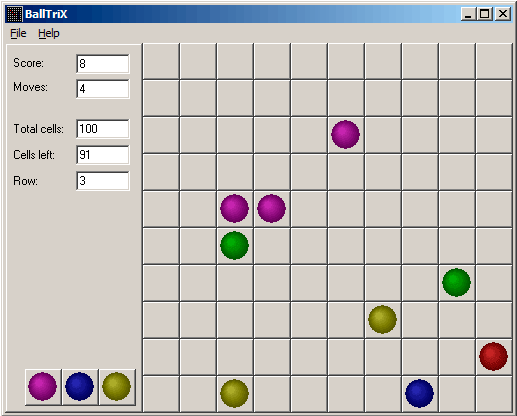
\includegraphics[scale=\FigScale]{examples/lines/1.png}
\caption{\RU{Обычный вид игры}\EN{How this game looks usually}}
\label{fig:lines_1}
\end{figure}

\clearpage
\myindex{\CStandardLibrary!rand()}
\RU{Посмотрим, сможем ли мы найти генератор псевдослучайных чисел и и сделать с ним одну шутку.}
\EN{So let's see, is it be possible to find the random generator and do some trick with it.}
\IDA \RU{быстро распознает стандартную функцию}\EN{quickly recognize the standard} \TT{\_rand} \RU{в}\EN{function in} 
\TT{balltrix.exe} \RU{по адресу}\EN{at} \TT{0x00403DA0}.
\IDA \RU{также показывает, что она вызывается только из одного места}\EN{also shows that it is called 
only from one place}:

\lstinputlisting{examples/lines/random.lst}

\RU{Назовем её}\EN{We'll call it} \q{random}.
\RU{Пока не будем концентрироваться на самом коде функции}\EN{Let's not to dive into this function's code yet}.

\RU{Эта функция вызывается из трех мест}\EN{This function is referred from 3 places}.

\RU{Вот первые два}\EN{Here are the first two}:

\lstinputlisting{examples/lines/1.lst}

\EN{Here is the third one}\RU{Вот третье}:

\lstinputlisting{examples/lines/2.lst}

\RU{Так что у функции только один аргумент}\EN{So the function has only one argument}.
\RU{10 передается в первых двух случаях и 5 в третьем.}
\EN{10 is passed in first two cases and 5 in third.}
\RU{Мы также можем заметить, что размер доски 10*10 и здесь 5 возможных цветов}\EN{We can also notice 
that the board has a size of 10*10 and there are 5 possible colors}.
\RU{Это оно}\EN{This is it}!
\RU{Стандартная функция}\EN{The standard} \TT{rand()} \RU{возвращает число в пределах}\EN{function returns 
a number in the} \TT{0..0x7FFF} \RU{и это неудобно, так что многие программисты пишут свою функцию,
возвращающую случайное число в некоторых заданных пределах}\EN{range and this is often inconvenient,
so many programmers implement their own random functions which returns a random number in a specified range}.
\RU{В нашем случае, предел это}\EN{In our case, the range is} $0..n-1$ \AndENRU $n$ \RU{передается как
единственный аргумент в функцию}\EN{is passed as the sole argument of the function}.
\RU{Мы можем быстро проверить это в отладчике}\EN{We can quickly check this in any debugger}.

\RU{Сделаем так, чтобы третий вызов функции всегда возвращал ноль}\EN{So let's fix the third function call to always return zero}.
\RU{В начале заменим три инструкции}\EN{First, we will replace three instructions} (\TT{PUSH/CALL/ADD}) 
\RU{на}\EN{by} \ac{NOP}s.
\RU{Затем добавим инструкцию}\EN{Then we'll add} \INS{XOR EAX, EAX}\RU{, для очистки регистра \EAX}\EN{ instruction, 
to clear the \EAX register}.

\lstinputlisting{examples/lines/fixed.lst}

\RU{Что мы сделали, это заменили вызов функции}\EN{So what we did is we replaced a call to the} \TT{random()} 
\RU{на код, всегда возвращающий ноль}\EN{function by a code which always returns zero}.

\clearpage
\RU{Теперь запустим}\EN{Let's run it now}:

\begin{figure}[H]
\centering
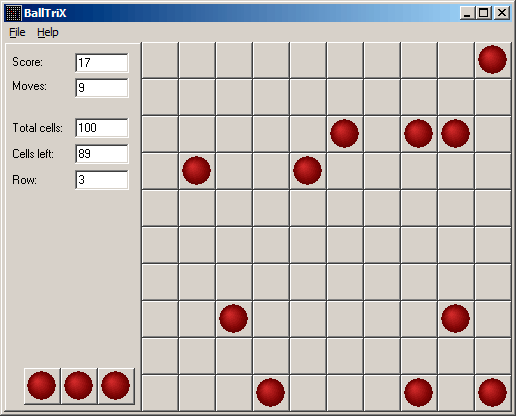
\includegraphics[scale=\FigScale]{examples/lines/2.png}
\caption{\RU{Шутка сработала}\EN{Practical joke works}}
\end{figure}

\RU{О да, это работает}\EN{Oh yes, it works}\footnote{\RU{Автор этой книги однажды сделал это как 
шутку для его сотрудников, в надежде что они перестанут играть. 
Надежды не оправдались.}\EN{Author of this book once did this as a joke for his coworkers with 
the hope that they would stop playing. They didn't.}}.

\RU{Но почему аргументы функции}\EN{But why are the arguments to the} \TT{random()} \RU{это глобальные 
переменные}\EN{functions global variables}?
\RU{Это просто потому что в настройках игры можно изменять размер доски, так что эти параметры не 
фиксированы}\EN{That's just because it's possible to change the board size in the game's settings, 
so these values are not hardcoded}.
\EN{The }10 \AndENRU 5 \RU{это просто значения по умолчанию}\EN{values are just defaults}.
